\chapter{A better KD-tree implementation}\label{ch:fkdtree}
In this chapter we describe a different implementation of a KD-tree that fixes the issues of the volume KD-tree explained in Section \ref{sec:volumeKdAssessment} and implements a search much more suitable to a highly parallel computation. The implementation is again wrote in \CC\ and CUDA for the GPU relevant parts.

\section{Build of a left-balanced KD-tree}
A left-balanced binary tree is a tree in which the leaves only occupy the leftmost positions in the last level. This positioning can be applied to the leaves of a KD-tree as well by chosing to assign the leaves of the tree to the leftmost available parent.\\
In practice this can be achieved by assigning the index of each node of the tree to a pre-determined value evaluated by the node's depth in the tree and its relative position among the other nodes at the same depth.\\
The KD-tree nodes are assigned to a binary tree, therefore each node has two children in the next layer and the number of nodes $N_d$ at a given depth $d$ can be evaluated as $N_d = 2^d$ where $d = 0$ is the depth of the root. Moreover the indeces of the children of a given node of index $I_p$ can also be simply evaluated to be $I_{left} = I_p \cdot 2$ and $I_{right} = I_p \cdot 2 + 1$. Using this knowledge we assign to the nodes of the tree a pre-determined index.\\
For this implementation of KD-tree we also drop the feature used in the volume KD-tree to assign a volume to each node of the tree. In this implementation each node of the tree corresponds to one point of the data set.\\
By exploiting the predictive placement of the tree's nodes we can also implement a build procedure that is iterative instead of recursive: an outer loop visits all the layers of the tree until all the leaves are created, inside another internal loop -that spans the tree horizontaly- creates one by one the children of the nodes at the current depth, assigning them the index that can be evaluated as powers of 2 as described by the above formula. The inner loops ends when all the children of the next depth are created, and the outer loop ends when each point of the data set is a node of the tree.\\
We determine the point to assign to each node by a sort performed along an axis similar to the one described in Paragraph \ref{sec:volumeKDBuild}, however in this implementation we realize that there is no reason to sort all the points in the range, what is needed, indeed, is to find the median point among them along the sorting axis, and then the points with the coordinate along the splitting axis smaller on one side and those with greater coordinates on the other side: the relative sorting in this two sets is irrelevant and can be avoided to gain some performance. The STL library provides a function that just does that: \textit{std::nth\_element} which we include in the build procedure.\\
Algorithm \ref{fkdtree_build} shows how we implemented the features described above.\\

\begin{algorithm}
\caption{The build of a left-balanced KD-tree}
\label{fkdtree_build}
\begin{algorithmic}
\Procedure{BuildKDTree}{numberOfPoints, points}
  \State pointsToEvaluate $\gets$ 0
  \For{(thisDepth $<$ maximumDepth)}
  \State axis $\gets$ thisDepth $\bmod$ 3 \Comment 0 = $x$, 1 = $y$, 2 = $z$
	  \For{ (thisIndex $<$ thisDepth$^2$)}
	  	\State medianValue $\gets$ pointsToEvaluate[thisIndex] / 2
	  	\State sortedPoints $\gets$ std::nth\_element(pointsInThisNode, medianValue)
	  	\State thisIndex $\gets$ medianValue
	  	\State tree[thisIndex] $\gets$ points[thisIndex]
	  	\State pointsToEvaluate[leftSon] $\gets$ sortedPoints[0,thisIndex)
	  	\State pointsToEvaluate[rightSon] $\gets$ sortedPoints[thisIndex, lastIndex]
	  \EndFor
  \EndFor
\EndProcedure
\end{algorithmic}
\end{algorithm}

\section{Iterative range search}
To perform a range search the algorithm takes a ``search box'' as argument for which it finds the points in the data set that are enclosed in it.\\
The search procedure, recursive by nature, is made iterative by exploiting the the predictable nodes placement described by the build procedure. Particularly, starting from the root node, the algorithm checks if the node -along the splitting axis defined by the node's depth- is greater than the search box maximum vertex, smaller of the minimum vertex or if it lies in the search box. When the node is greater than the search box the search proceeds on the node's left-child, when is smaller on the right-child and when it lies within the search box both children are considered for the next step in the search and the node is recorded as a nearest neighbor and will not be checked again.\\
In order to make the above procedure iterative, avoiding the recursion, a loop is performed on all the nodes to compare the search box against. The iteration is initialized by adding to a \textit{queue} the root node index. The loop starts and compare the search box against the root, then one or both of its childrens are added to the queue while the node compared is removed from the queue. The next iteration of the cycle will compare the search box against the last element of the queue (e.g. the node(s) added on the previous step) and remove it from the queue while adding whichever children the search must proceed on. The loop repeats until the queue is empty which means that the leaves are all reached and all the nearest neighbors recorded.\\

\subsection{Fast bitwise operations}
At every step of the search the axis along which the current node has been created must be known. It can be easily deduced by knowing the depth of the tree the node is situated at, which in turns could be saved as part of the information of the node, however we decided against it to reduce to the bare minimum the memory footprint of the array of nodes. The depth of the node in the tree, indeed, can be evaluated from the node index $I$ by inverting the formula described in the previous Section, that is: $d = \lfloor log_2(I) \rfloor$ which in \CC\ can be easily implemented with the embedded C functions as: \code{d = floor(log2(I))}.\\
However we analysed the performance of the above code and found that it is relatively expensive in execution time. Therefore we replaced the code based on the C functions with a custom function leveraging the bitwise operators: \code{((unsigned int) (31 - \_\_builtin\_clz( I | 1) ))}. Starting from the inner parts the \code{I | 1} cosiders the integer representing the index of the node as a sequence of bits and does the $OR$ with the bit $1$, this ensures that the function works also in the case of $I = 0$. Then \code{\_\_builtin\_clz()} counts the number of leading zeroes in the index of the node when represented in binary form. The total number of bits representing an \code{unsigned int} in most common computer architectures is 32, therefore subtracting the number of leading zeroes of the index to 32 gives the logarithm in base two of the index. Subtracting one to that number and then performing the cast to \code{unsigned int} performs the equivalent of the \code{floor()} operation giving the expected result.\\
This seemingly harmless substitution in the code resulted in a very tangible increase in performance being up to ten times faster than the code using the C functions.\\
The implementation of the range search is showed in Algorithm \ref{fkdtree_search}.\\

\begin{algorithm}
\caption{Range search of the left-balanced KD-tree}
\label{fkdtree_search}
\begin{algorithmic}
\Procedure{SearchKDTree}{searchBox}
  \State nodesToVisit $\gets$ 0
  \While{(nodesToVisit)}
  	\State indexToCheck $\gets$ nodesToVisit[last]
  	\State thisDepth $\gets$ \textbf{FLOOR\_LOG2}(indexToCheck) \Comment as explained above
	\State axis $\gets$ thisDepth $\bmod$ 3 \Comment 0 = $x$, 1 = $y$, 2 = $z$
	\If{(searchBox[axis][min] $<=$ indexToCheck[axis] \\ \hspace{4em} \textbf{AND} searchBox[axis][max] $>=$ indexToCheck[axis])}
		\State nodesToVisit $\gets$ leftChild, rightChild
		\State nearestNeighborsResult $\gets$ indexToCheck
	\ElsIf{(searchBox[axis][max] $<=$ indexToCheck[axis])}
		\State nodesToVisit $\gets$ leftChild
	\Else
		\State nodesToVisit $\gets$ rightChild
	\EndIf		
	\State nodesToVisit $\textit{remove}$ indexToCheck
  \EndWhile
  \State \textbf{return} nearestNeighborsResult
\EndProcedure
\end{algorithmic}
\end{algorithm}

\section{Validation}
We implemented the KD-tree algorithm in \CC\ and validated it with the same technique described in Section \ref{sec:volume_kdtree_validation}, using uniformly distributed random points and comparing the search results with the \textit{naive} method.\\
As an additional validation and debug tools we implemented two recursive functions for the build and the range search respectively.
The first, through the classic recursion, verify that the nodes have the correct relative positioning among them. While the second, again recursively, verify that when searching for a single point of the data set used to build the tree, said point is indeed found in the leaf it is supposed to be.\\

\section{GPU porting}
We focus our attention on parallelizing the range search part of the algorithm and run it on a GPU. We expect to gain a significative increase in performance by running the all nearest neighbors searches in parallel assigning one search box to one CUDA thread and executing several thousand (depending on the actual GPU used) threads at the same time.\\
In order to port the algorithm described in \ref{fkdtree_search} to CUDA there are some obstacles to get around first.\\

\subsection{GPU queue}
CUDA does not support STL containers and does not provide a variable size queue (at least in version 7.5 used in this work). Therefore we made our own implementation to save the nodes indices to visit in each loop cycle.\\
The motivations to have a variable size queue are mainly two: the tree could be arbitrarily long and if the visited node index was not removed at each cycle the size of the array containing the visited nodes could become too big for the very limited registry memory each CUDA core has access to (see Section \ref{sec:gpu_arch}). The second reason is that by having a dynamic size it is always known which is the last element of the queue allowing the search to access it at every cycle and then remove it.\\
The implementation is reported in Appendix \ref{ch:appendixFKDTree}.

\subsection{CUDA streams}
The array of search boxes and the array of the nodes (the tree structure) must be both moved on the GPU memory before executing the code that performs the range search, also, the array of the index of the nearest neighbors must be copied back on the host computer once the search is completed. The time necessary to perform those copy can be a relevant fraction of the total time spent for the range search.\\
Nvidia's GPUs provides a feature that can help mitigate the time cost of copying the data to and from the device. Recent Nvidia GPUs are able to copy data to the device, from the device and execute code at the same time. Clearly to have an output to copy back on the host machine the code execution must have ran which, in turn, must have had access to the input data copied on the GPU device. Therefore to profit of the feature the whole search process must be split in what CUDA calls \textit{streams}, inside every stream the copy to the device, the execution and the copy from the device are executed sequentially, however different streams are asyncronous and indipendent. So, for instance, suppose to have two streams: the first stream begins to copy its portion of data on the device, once it is done its execution begins but, at the same time, the copy of the data on the device of the second stream begins. Likewise the stream 1 can then copy the output back to the host machine while stream 2 is still executing the code.\\
Figure \ref{cuda_streams} shows how the interleaving of the streams can ``hide'' the cost of the memory management.\\

\begin{figure}
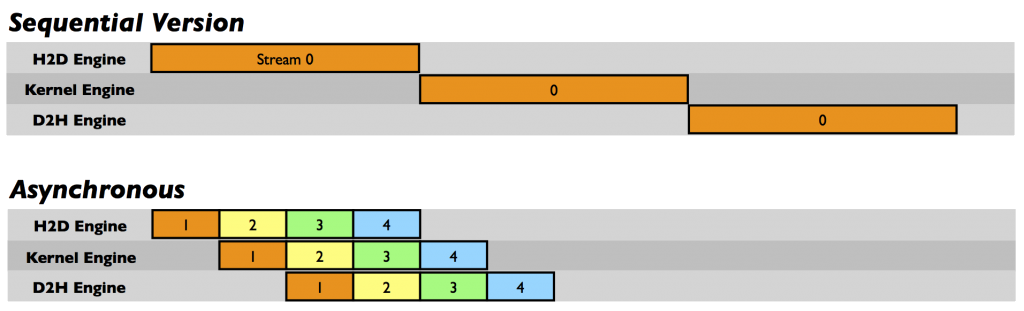
\includegraphics[width=\textwidth]{fkdtree/cuda_streams.png}
\caption{Interleaving of four asyncronous CUDA streams. H2D: host to device process, D2H: device to host, Kernel: code execution.}
\label{cuda_streams}
\end{figure}

We implemented in the search algorithm the possibility to split the all nearest neighbors search in an arbitrary number of CUDA streams to evaluate which number of streams yields the best performance.\\

\section{Performance analysis}
To evaluate the performance of this implementation we use the same method applied to the volume KD-tree used in Section \ref{sec:volumeKd_performance} with further investigation where required.\\

\subsection{Uniform random distribution}
The first set of tests are performed by building the KD-tree off a uniform random distribution of points. The data sets are produced with a number of points ranging from $2 \times 10^4$ to $5 \times 10^5$.\\
We measure the time spent building the tree, the search times differences for the GPU parallel code with different number of CUDA streams, the search times of the CPU sequential code and the speedup between the two.\\
Figure \ref{fkdtree_build_times} shows the time spent building the KD-tree for the various number of data set points.\\

\begin{figure}
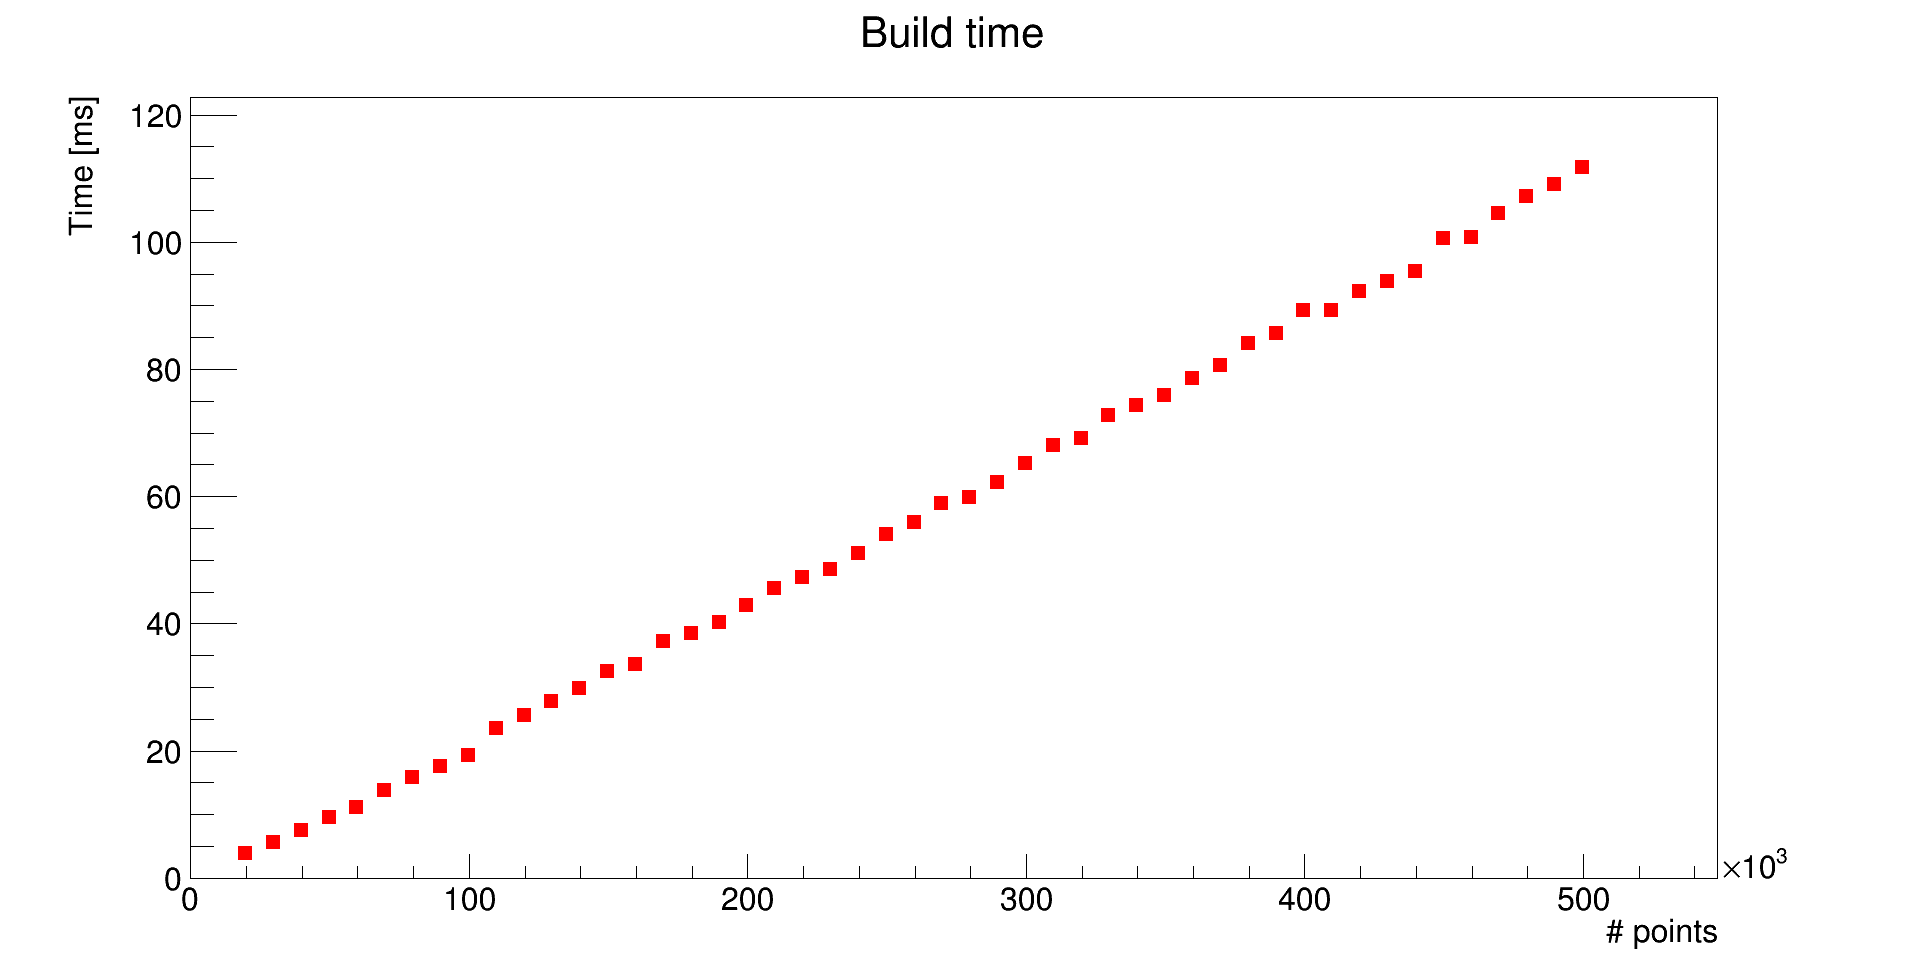
\includegraphics[width=\textwidth]{fkdtree/fkdBuildTimes.png}
\caption{Time spent by the build of the KD-tree.}
\label{fkdtree_build_times}
\end{figure}

Figure \ref{fkdtree_streams} shows the relative performance gain of the search performed with 2 to 16 CUDA streams with respect to the single stream for a number of generated points between $6 \times 10^4$ to $5 \times 10^5$.\\
\begin{figure}
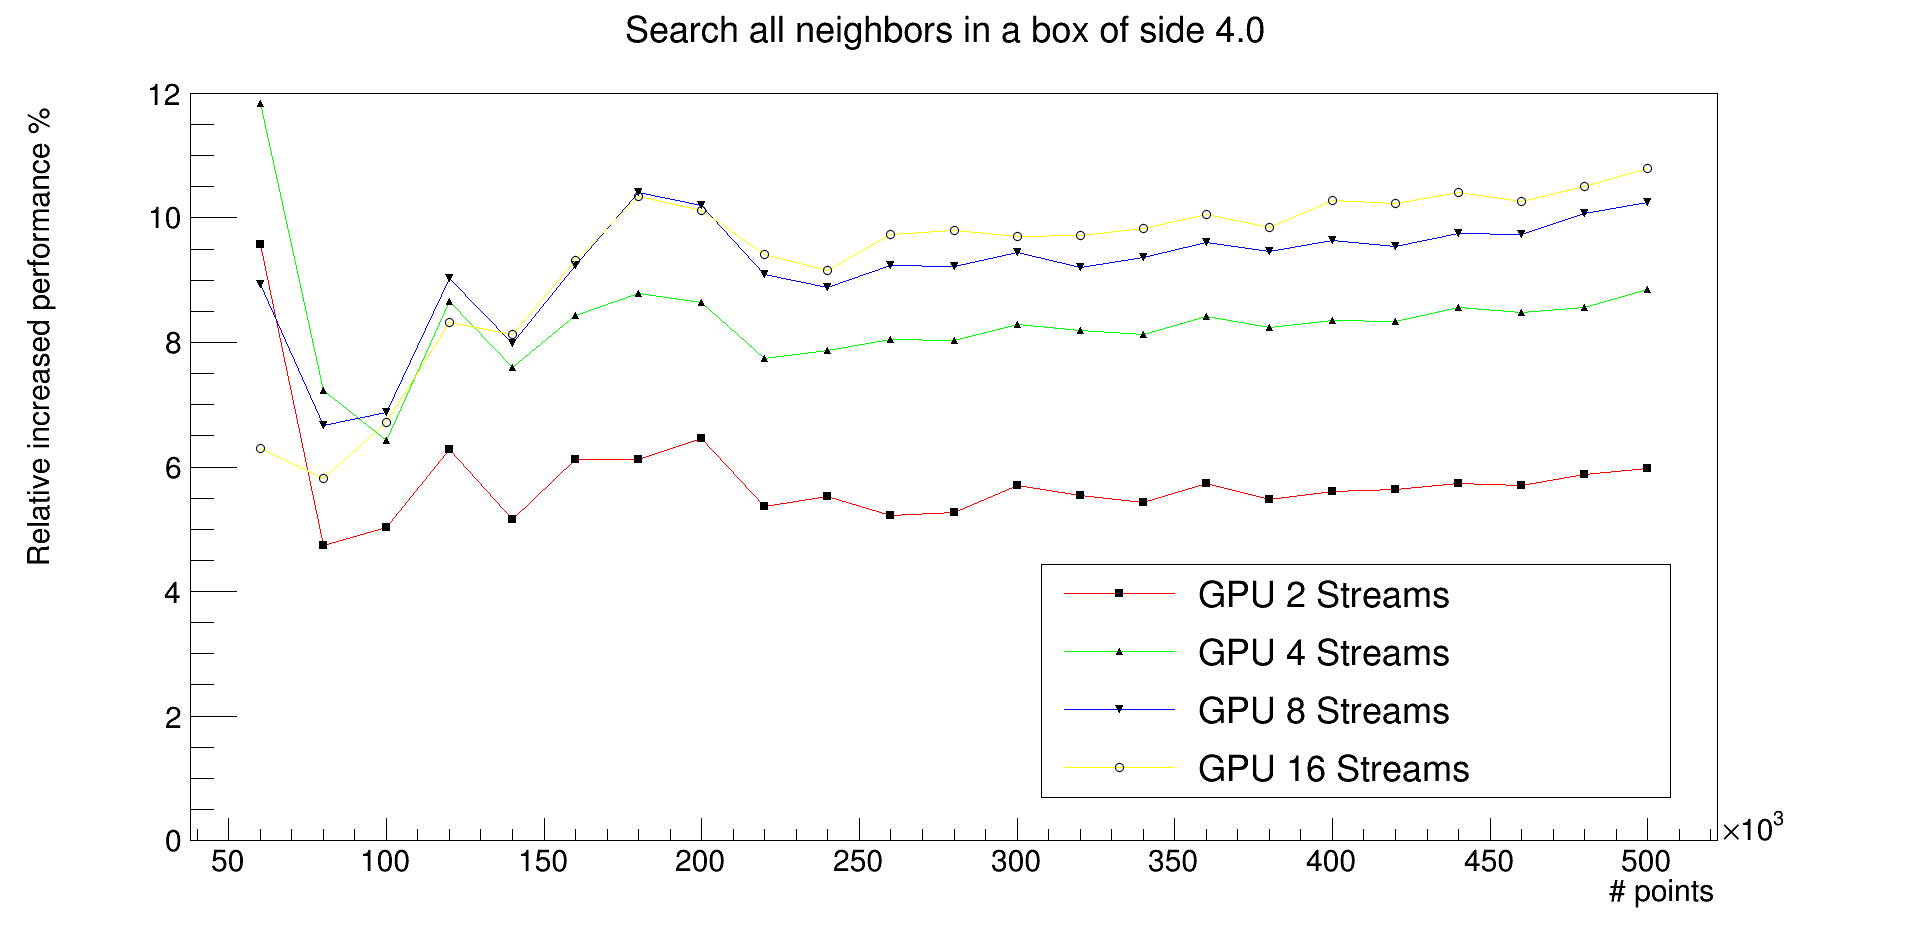
\includegraphics[width=\textwidth]{fkdtree/fkdStreams.png}
\caption{Relative performance gain between multiple CUDA streams with respect to the single stream.}
\label{fkdtree_streams}
\end{figure}

Following the results of the streams performance analysis we chose to use 8 CUDA streams to evaluate the performance of the GPU search with respect to the CPU one.\\

Figure \ref{fkdtree_search_times} shows the timings of the CPU sequential search and the GPU parallel one in the full range of the generated data sets, with the times shown in logarithmic scale.

\begin{figure}
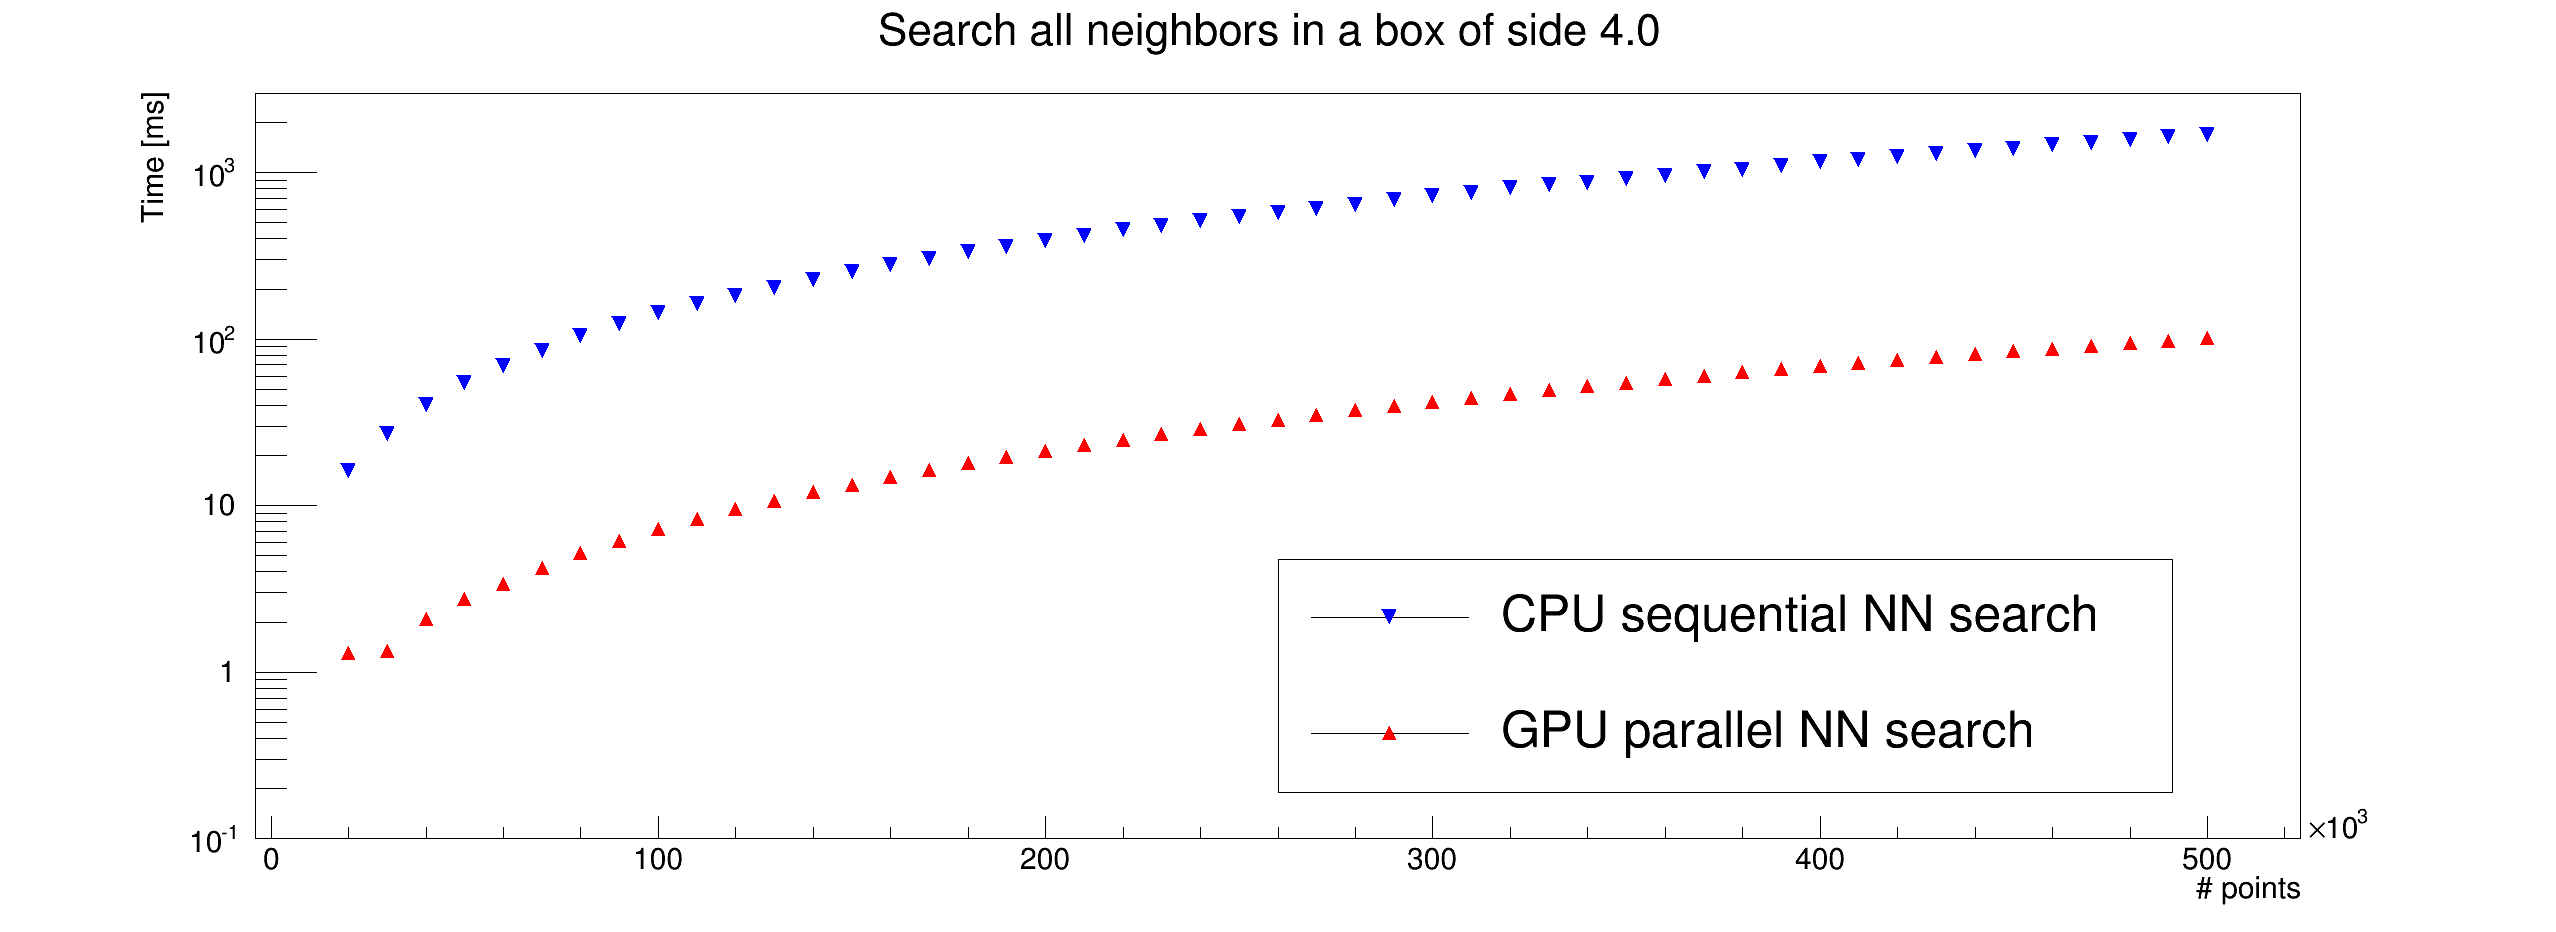
\includegraphics[width=\textwidth]{fkdtree/fkdSearchTimes.png}
\caption{Search times for CPU sequential and GPU parallel code.}
\label{fkdtree_search_times}
\end{figure}

Some selected timings are reported in Table \ref{fkdtree_times_tab}.\\

\begin{center}
\begin{table}[h]
\begin{tabular}{ c || r r r r r r r r r r }
Points ($10^{3}$) & 50 & 100 & 150 & 200 & 250 & 300 & 350 & 400 & 450 & 500 \\
\hline
CPU ($\unit{ms}$) & 54 & 142 & 253 & 384 & 539 & 714 & 907 & 1143 & 1384 & 1682 \\
GPU ($\unit{ms}$) & 3 & 7 & 13 & 21 & 31 & 42 & 54 & 68 & 84 & 101 \\
\end{tabular}
\caption{Selected search times for CPU sequential and GPU parallel code.}
\label{fkdtree_times_tab}
\end{table}
\end{center}

Lastly Figure \ref{fkdtree_speedup} shows the speedup between the two search methods.\\
\begin{figure}
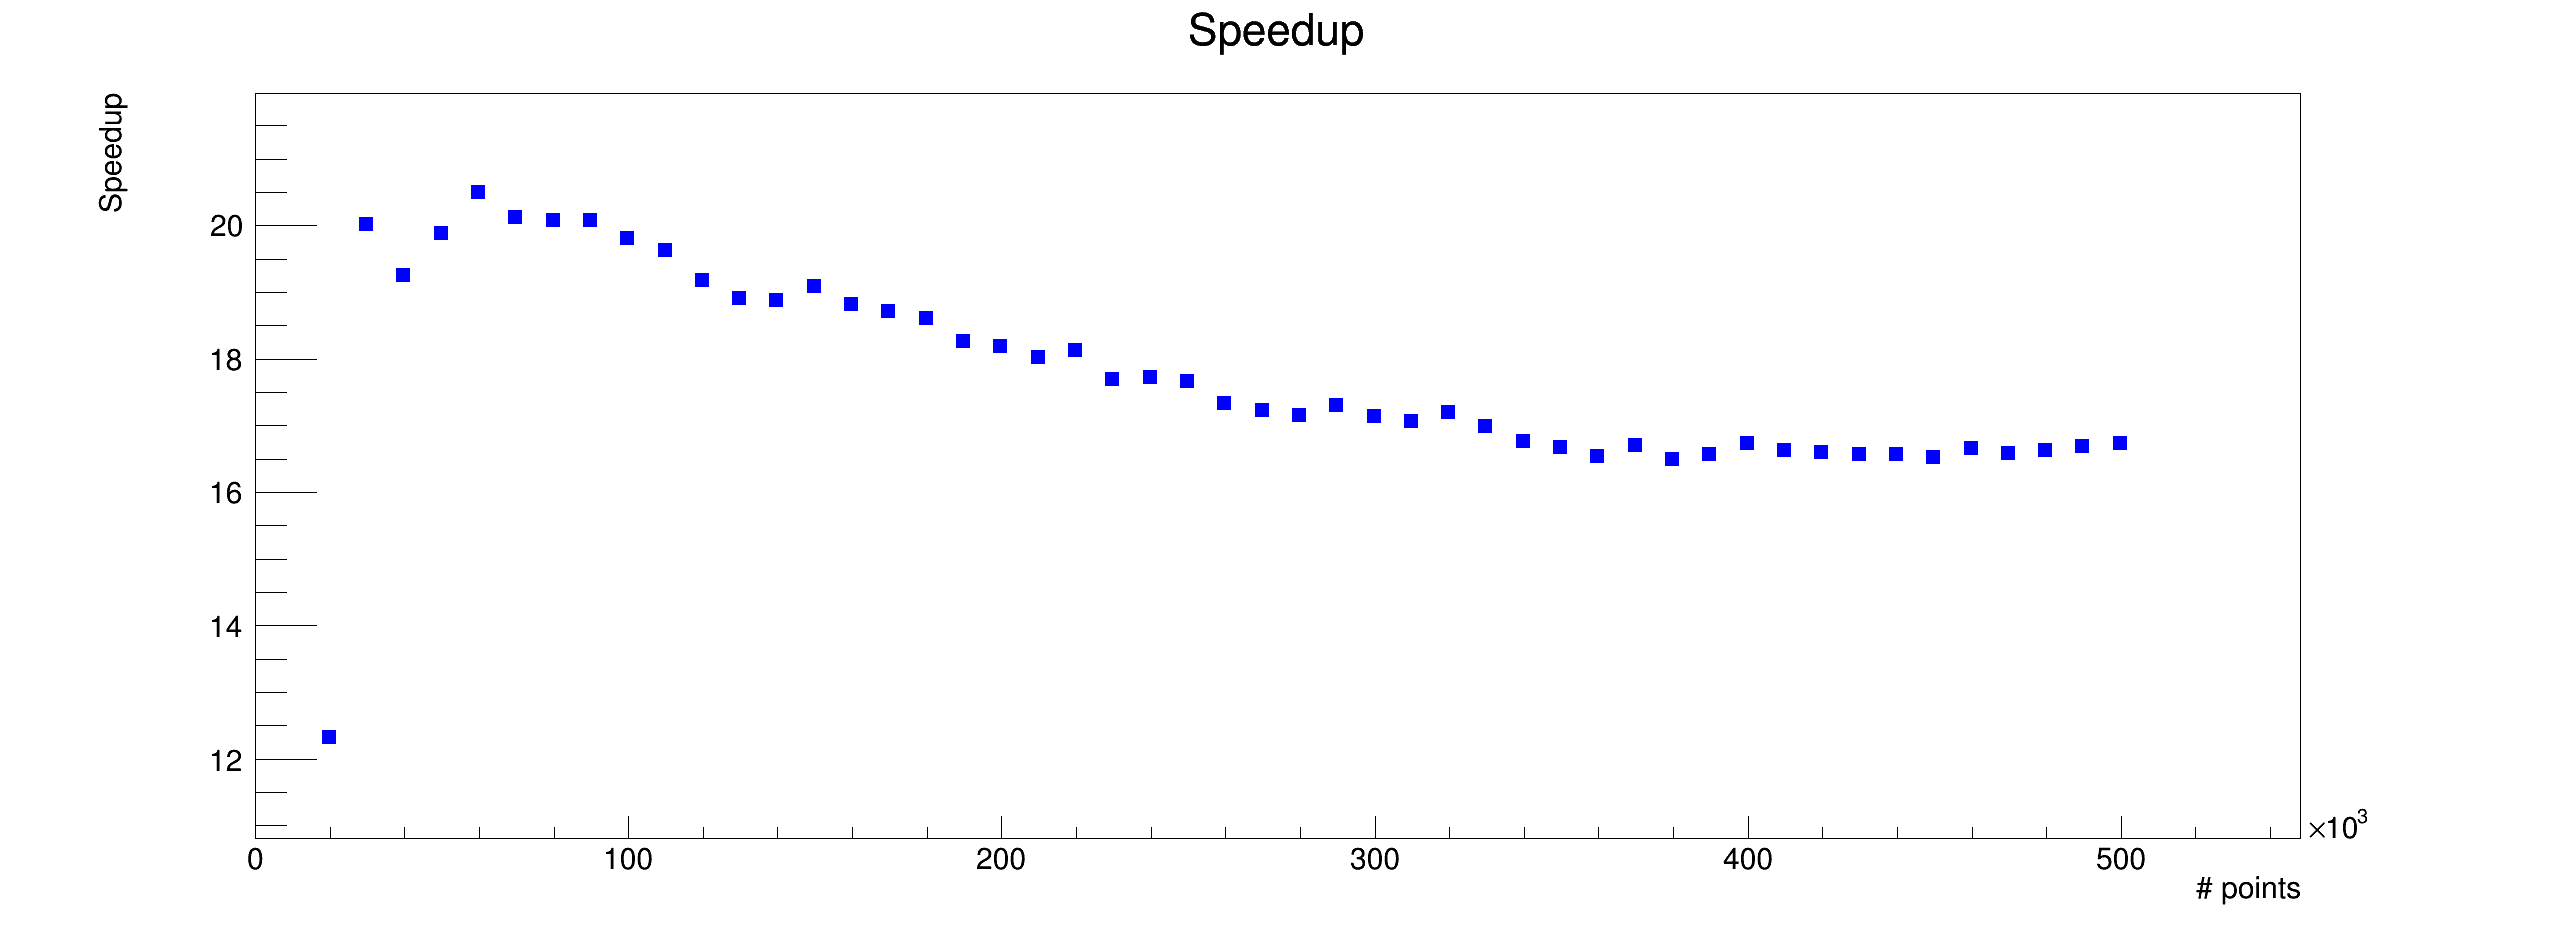
\includegraphics[width=\textwidth]{fkdtree/fkdSpeedup.png}
\caption{Speedup between CPU sequential and GPU parallel code.}
\label{fkdtree_speedup}
\end{figure}

\subsection{HGCAL simulated RecHits}

\section{Algorithm assessment}